\usetikzlibrary{automata,arrows}
\section*{Problem 6}
	\begin{enumerate} [(a)]
		\item \begin{proof} [Solution]
			\mbox{}\\
			\begin{center}
				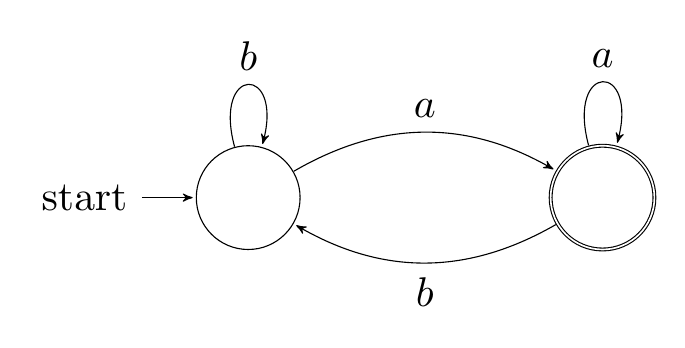
\begin{tikzpicture}
					[>=stealth', shorten >=1pt, auto, node distance=3cm, scale=1.5, transform shape]
					\node[initial, state] (A) {};
					\node[state,accepting] (C) [right of=A] {};
					\path[->] (A) edge [bend left] node [align=center] {$a$} (C)
					(C) edge [bend left] node [align=center] {$b$} (A)
					(C) edge [loop above] node [align=center] {$a$} (C)
					(A) edge [loop above] node [align=center] {$b$} (A);
				\end{tikzpicture}
			\end{center}
		\end{proof}
		\item \begin{proof} [Solution]
			\mbox{}\\
			\begin{center}
				\begin{tikzpicture}
					[>=stealth', shorten >=1pt, auto, node distance=3cm, scale=1.5, transform shape]
					\node[initial, state] (A) {};
					\node[state] (B)[above right of=A] {};
					\node[state,accepting] (C) [right of=A] {};
					\path[->] (A) edge node [align=center] {$a$} (C)
					(A) edge node [align=center] {$b$} (B)
					(C) edge [loop right] node [align=center] {$a,b$} (C)
					(B) edge [loop right] node [align=center] {$a,b$} (B);
				\end{tikzpicture}
			\end{center}
		\end{proof}
		\item \begin{proof} [Solution]
			\mbox{}\\
			\begin{center}
				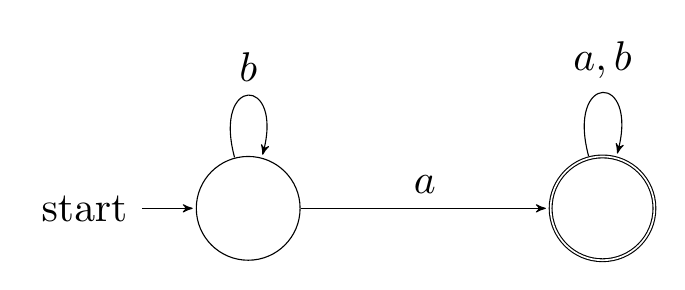
\begin{tikzpicture}
					[>=stealth', shorten >=1pt, auto, node distance=3cm, scale=1.5, transform shape]
					\node[initial, state] (A) {};
					\node[state,accepting] (C) [right of=A] {};
					\path[->] (A) edge node [align=center] {$a$} (C)
					(C) edge [loop above] node [align=center] {$a,b$} (C)
					(A) edge [loop above] node [align=center] {$b$} (A);
				\end{tikzpicture}
			\end{center}
		\end{proof}
		\newpage
		\item \begin{proof} [Solution]
			\mbox{}\\
			\begin{center}
				\begin{tikzpicture}
					[>=stealth', shorten >=1pt, auto, node distance=3cm, scale=1.2, transform shape]
					\node[initial, state] (A) {};
					\node[state] (B) [above right of=A] {};
					\node[state,accepting] (C) [below right of=B] {};
					\node[state] (D) [below right of=A] {};
					\path[->] (A) edge node [align=center] {$a$} (D)
					(A) edge node [align=center] {$b$} (B)
					(B) edge node [align=center] {$a$} (C)
					(B) edge node [align=center] {$b$} (D)
					(C) edge [loop right] node [align=center] {$a,b$} (C)
					(D) edge [loop right] node [align=center] {$a,b$} (D);
				\end{tikzpicture}
			\end{center}
		\end{proof}
		\item \begin{proof} [Solution]
			\mbox{}\\
			\begin{center}
				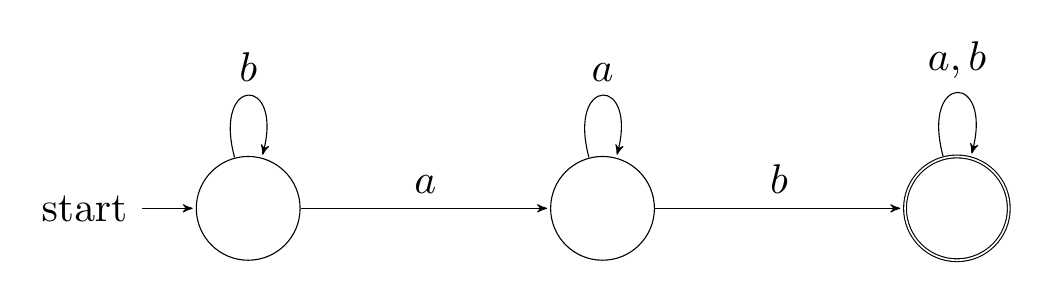
\begin{tikzpicture}
					[>=stealth', shorten >=1pt, auto, node distance=3cm, scale=1.5, transform shape]
					\node[initial, state] (A) {};
					\node[state] (B) [right of=A] {};
					\node[state,accepting] (C) [right of=B] {};
					\path[->] (A) edge node [align=center] {$a$} (B)
					(B) edge node [align=center] {$b$} (C)
					(C) edge [loop above] node [align=center] {$a,b$} (C)
					(A) edge [loop above] node [align=center] {$b$} (A)
					(B) edge [loop above] node [align=center] {$a$} (B);
				\end{tikzpicture}
			\end{center}
		\end{proof}
	\end{enumerate}